\documentclass{article}
\usepackage{import}
\subimport*{../../}{macro}

\setlength\parindent{0px}

\begin{document}
\setcounter{aprob}{0}
\setcounter{bprob}{0}
\title{Homework \#1}
\author{
    \normalsize{CSE 446/546: Machine Learning}\\
    \normalsize{Profs. Jamie Morgenstern and Simon Du}\\
    \normalsize{Due: \textbf{Wednesday} October 20, 2021 11:59pm}\\
    \normalsize{\textbf{A:} 59 points, \textbf{B:} 30 points}
}
\date{{}}
\maketitle

\noindent Please review all homework guidance posted on the website before submitting to GradeScope. Reminders:
\begin{itemize}
    \item Make sure to read the ``What to Submit'' section following each question and include all items.
    \item Please provide succinct answers and supporting reasoning for each question. Similarly, when discussing experimental results, concisely create tables and/or figures when appropriate to organize the experimental results. All explanations, tables, and figures for any particular part of a question must be grouped together.
    \item For every problem involving generating plots, please include the plots as part of your PDF submission.
    \item When submitting to Gradescope, please link each question from the homework in Gradescope to the location of its answer in your homework PDF. Failure to do so may result in deductions of up to \points{5}. For instructions, see \url{https://www.gradescope.com/get_started#student-submission}.
    \item Please recall that B problems, indicated in \boxed{\textrm{boxed text}}, are only graded for 546 students, and that they will be weighted at most 0.2 of your final GPA (see website for details). In Gradescope there is a place to submit solutions to A and B problems separately. You are welcome to create just a single PDF that contains answers to both, submit the same PDF twice, but associate the answers with the individual questions in Gradescope. 
    \item If you collaborate on this homework with others, you must indicate who you worked with on your homework. Failure to do so may result in accusations of plagiarism.
    \item For every problem involving code, please include the code as part of your PDF for the PDF submission \emph{in addition to} submitting your code to the separate assignment on Gradescope created for code. Not submitting all code files will lead to a deduction of \points{1}.  
\end{itemize}

Not adhering to these reminders may result in point deductions. \\

% \textcolor{red}{\textbf{Changelog:}}

% \begin{itemize}
%     \item \textbf{Date:} Changed This.
% \end{itemize}

\clearpage{}


% Start of Problems:

\section*{Short Answer and ``True or False'' Conceptual questions}
\begin{aprob}
    The answers to these questions should be answerable without referring to external materials.  Briefly justify your answers with a few words.
    \begin{enumerate}
        \item\points{2} In your own words, describe what bias and variance are? What is bias-variance tradeoff?
        \item \points{2} What \textbf{typically} happens to bias and variance when the model complexity increases/decreases?
        \item \points{1} True or False: A learning algorithm will always generalize better if we use fewer features to represent our data. 
        \item \points{2} True or False: Hyperparameters should be tuned on the test set. Explain your choice and detail a procedure for hyperparameter tuning.
        \item \points{1} True or False: The training error of a function on the training set provides an overestimate of the true error of that function.
    \end{enumerate}
    \subsubsection*{What to Submit:}
    \begin{itemize}
        \item \textbf{Parts c-e:} True or False
        \item \textbf{Parts a-e:} Brief (2-3 sentence) explanation
    \end{itemize}
\end{aprob}

\section*{Maximum Likelihood Estimation (MLE)}

\begin{aprob}
    You're the Reign FC manager, and the team is five games into its 2021 season. The number of goals scored by the team in each game so far are given below:
    
    \[
      [2, 4, 6, 0, 1].
    \]
    Let's call these scores $x_1, \dots, x_5$. Based on your (assumed iid) data, you'd like to build a model to understand how many goals the Reign are likely to score in their next game. You decide to model the number of goals scored per game using a \emph{Poisson distribution}. Recall that the Poisson distribution with parameter $\lambda$ assigns every non-negative integer $x = 0, 1, 2, \dots$ a probability given by
    \[
      \mathrm{Poi}(x | \lambda) = e^{-\lambda} \frac{\lambda ^ x}{x!}.
    \]
    
    \begin{enumerate}
        \item \points{5} Derive an expression for the maximum-likelihood estimate of the parameter $\lambda$ governing the Poisson distribution in terms of goal counts for the first $n$ games: $x_1, \dots, x_n$. (Hint: remember that the log of the likelihood has the same maximizer as the likelihood function itself.)
        \item \points{2} Give a numerical estimate of $\lambda$ after the first five games. Given this $\lambda$, what is the probability that the Reign score $6$ goals in their next game?
        \item \points{2} Suppose the Reign score 8 goals in their 6th game. Give an updated numerical estimate of $\lambda$ after six games and compute the probability that the Reign score $6$ goals in their 7th game.
    \end{enumerate}
    \subsubsection*{What to Submit:}
    \begin{itemize}
        \item \textbf{Part a:} An expression for the MLE of $\lambda$ after $n$ games and relevant derivation
        \item \textbf{Parts b-c:} A numerical estimate for $\lambda$ and the probability that the Reign score 6 next game.
    \end{itemize}
\end{aprob}

\begin{aprob}
    \points{10} \textit{(Optional Background)} In World War 2, the Allies attempted to estimate the total number of tanks the Germans had manufactured by looking at the serial numbers of the German tanks they had destroyed. The idea was that if there were $n$ total tanks with serial numbers $\{1,\dots,n\}$ then its reasonable to expect the observed serial numbers of the destroyed tanks constituted a uniform random sample (without replacement) from this set. The exact maximum likelihood estimator for this so-called \emph{German tank problem} is non-trivial and quite challenging to work out (try it!). For our homework, we will consider a much easier problem with a similar flavor.\\

    Let $x_1,\dots,x_n$ be independent, uniformly distributed on the continuous domain $[0,\theta]$ for some $\theta$. What is the Maximum likelihood estimate for $\theta$?
    \subsubsection*{What to Submit:}
    \begin{itemize}
        \item An expression for the MLE of $\theta$ after $n$ games and relevant derivation.
    \end{itemize}
\end{aprob}

\section*{Overfitting}
\begin{bprob}
    Suppose we have $N$ labeled samples $S = \{(x_i,y_i)\}_{i=1}^N$ drawn i.i.d. from an underlying distribution $\mathcal{D}$. Suppose we decide to break this set into a set $S_{\textrm{train}}$ of size $N_{\textrm{train}}$ and a set $S_{\textrm{test}}$ of size $N_{\textrm{test}}$ samples for our training and test set, so $N = N_{\textrm{train}} + N_{\textrm{test}}$, and $S = S_{\textrm{train}} \cup S_{\textrm{test}}$.  Recall the definition of the true least squares error of $f$:
    \[
      \epsilon(f) = 
      \mathbb{E}_{(x,y) \sim \mathcal{D}} [ (f(x) -y)^2 ],
    \]
    where the subscript $(x,y) \sim \mathcal{D}$ makes clear that our input-output pairs are sampled according to $\mathcal{D}$. Our training and test losses are defined as:
    \begin{align*}
        \widehat{\epsilon}_{\textrm{train}}(f) &=
        \frac{1}{N _{\textrm{train}}} \sum_{(x,y)\in S_{\textrm{train}}}     (f(x) -y)^2\\
        \widehat{\epsilon}_{\textrm{test}}(f) &=
        \frac{1}{N _{\textrm{test}}} \sum_{(x,y)\in S_{\textrm{test}}}     (f(x) -y)^2  
    \end{align*}
    We then train our algorithm (for example, using linear least squares regression) using the training set to obtain $\widehat{f}$.
    
    \begin{enumerate}
        \item \points{3} (bias: the test error) For all fixed $f$ (before we've seen any data) show that
        \[
        \mathbb{E}_{\textrm{train}}[ \widehat{\epsilon}_{\textrm{train}}(f) ] = \mathbb{E}_{\textrm{test}}[ \widehat{\epsilon}_{\textrm{test}}(f) ] = \epsilon(f).
        \]
        Use a similar line of reasoning to show that the test error is an unbiased estimate of our true error for $\hat{f}$. Specifically, show that:
        \[
          \mathbb{E}_{\textrm{test}}[\widehat{\epsilon}_{\textrm{test}}(\widehat{f})] = \epsilon(\widehat{f})
        \]
        \item \points{4} (bias: the train/dev error) Is the above equation true (in general) with regards to the training loss? Specifically, does $\mathbb{E}_{\textrm{train}}[\widehat{\epsilon}_{\textrm{train}}(\widehat{f})]$ equal $\epsilon(\widehat{f})$? If so, why? If not, give a clear argument as to where your previous argument breaks down.
        \item \points{8} Let $\mathcal{F} = (f_1, f_2,\dots)$ be a collection of functions and let $\widehat{f}_{\textrm{train}}$ minimize the training error such that $\widehat{\epsilon}_{\textrm{train}}(\widehat{f}_{\textrm{train}}) \leq \widehat{\epsilon}_{\textrm{train}}(f)$ for all $f \in \mathcal{F}$.
        Show that
        \begin{align*}
            \mathbb{E}_{\text{train}}[ \widehat{\epsilon}_{\textrm{train}}(\widehat{f}_{\textrm{train}}) ] \leq \mathbb{E}_{\text{train,test}}[ \widehat{\epsilon}_{\textrm{test}}(\widehat{f}_{\textrm{train}}) ].
        \end{align*}
        (Hint: note that
        \begin{align*}
            \mathbb{E}_{\text{train,test}}[ \widehat{\epsilon}_{\textrm{test}}(\widehat{f}_{\textrm{train}}) ] &= \sum_{f \in \mathcal{F}} \mathbb{E}_{\text{train,test}}[ \widehat{\epsilon}_{\textrm{test}}(f) \1\{ \widehat{f}_{\textrm{train}} = f\}] \\
            &= \sum_{f \in \mathcal{F}} \mathbb{E}_{\text{test}}[ \widehat{\epsilon}_{\textrm{test}}(f) ] \mathbb{E}_{\text{train}}[ \1\{\widehat{f}_{\textrm{train}} = f \}]\\
            &= \sum_{f \in \mathcal{F}} \mathbb{E}_{\text{test}}[ \widehat{\epsilon}_{\textrm{test}}(f) ] \P_{\text{train}}(\widehat{f}_{\textrm{train}} = f )
        \end{align*}
        where the second equality follows from the independence between the train and test set.)
        \newline
    \end{enumerate}
    \subsubsection*{What to Submit:}
    \begin{itemize}
        \item \textbf{Part a} Proof
        \item \textbf{Part b} Brief Explanation (3-5 sentences)
        \item \textbf{Part c} Proof
    \end{itemize}
\end{bprob}

\section*{Polynomial Regression}
{\bf Relevant Files}\footnote{{\bf Bold text} indicates files or functions that you will need to complete; you should not need to modify any of the other files.}
\vspace{-1.2em}
\begin{multicols}{2}
    \begin{itemize}[noitemsep,nolistsep]
        \item \texttt{\bf polyreg.py}
        \item \texttt{linreg\_closedform.py}
        \item \texttt{test\_polyreg\_univariate.py}
        \item \texttt{test\_polyreg\_learningCurve.py}
        \item \texttt{data/polydata.dat}
    \end{itemize}
\end{multicols}

\begin{aprob}
    \points{10} Recall that polynomial regression learns a function $h_{\bm{\theta}}(x) = \theta_0 + \theta_1 x + \theta_2 x^2 + \ldots + \theta_d x^d$, where $d$ represents the polynomial's highest degree.  We can equivalently write this in the form of a  linear model with $d$ features
    \begin{equation}
        h_{\bm{\theta}}(x) = \theta_0 + \theta_1 \phi_1(x)  + \theta_2 \phi_2(x)  + \ldots + \theta_d \phi_d(x)  \enspace ,
    \end{equation}
    using the basis expansion that $\phi_j(x) = x^j$.  Notice that, with this basis expansion, we obtain a linear model where the features are various powers of the single univariate $x$.  We're still solving a linear regression problem, but are fitting a polynomial function of the input.\\
    
    Implement regularized polynomial regression in \texttt{polyreg.py}.  You may implement it however you like, using gradient descent or a closed-form solution.  However, I would recommend the closed-form solution since the data sets are small; for this reason, we've included an example closed-form implementation of linear regression in \texttt{linreg\_closedform.py} (you are welcome to build upon this implementation, but make CERTAIN you understand it, since you'll need to change several lines of it).  You are also welcome to build upon your implementation from the previous assignment, but you must follow the API below.  Note that all matrices are actually 2D numpy arrays in the implementation.\\
    
    \begin{itemize}[noitemsep, nolistsep]
        \item \texttt{\_\_init\_\_(degree=1, regLambda=1E-8)} : constructor with arguments of $d$ and $\lambda$
        \item \texttt{fit(X,Y)}: method to train the polynomial regression model
        \item \texttt{predict(X)}: method to use the trained polynomial regression model for prediction
        \item \texttt{polyfeatures(X, degree)}: expands the given $n \times 1$ matrix $X$ into an $n \times d$ matrix of polynomial features of degree $d$.  Note that the returned matrix will not include the zero-th power.\\
    \end{itemize}
    
    Note that the \texttt{polyfeatures(X, degree)} function maps the original univariate data into its higher order powers.  Specifically, $X$ will be an $n \times 1$ matrix $(X \in \mathbb{R}^{n \times 1})$ and this function will return the polynomial expansion of this data, a $n \times d$ matrix.  Note that this function will {\bf not} add in the zero-th order feature (i.e., $x_0 = 1$).  You should add the $x_0$ feature separately, outside of this function, before training the model.

    \begin{wrapfigure}{R}{0.42\textwidth}
        \centering
        \vspace{-1em}
        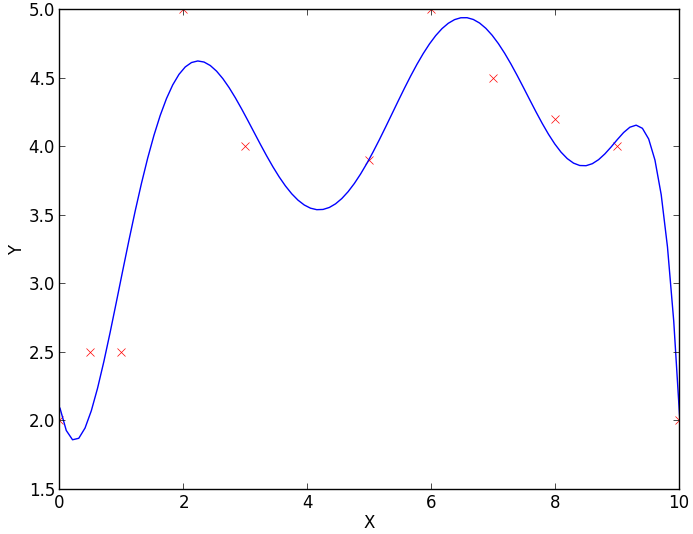
\includegraphics[width=0.4\textwidth]{../img/polyregDegree8.png}
        \vspace{-1em}
        \caption{Fit of polynomial regression with $\lambda = 0$ and $d = 8$}\label{fig:polyregUnivariate}
        \vspace{-2em}
    \end{wrapfigure}

    By not including the $x_0$ column in the matrix \texttt{polyfeatures()}, this allows the \texttt{polyfeatures} function to be more general, so it could be applied to multi-variate data as well. (If it did add the $x_0$ feature, we'd end up with multiple columns of 1's for multivariate data.)\\
    
    Also, notice that the resulting features will be badly scaled if we use them in raw form.  For example, with a polynomial of degree $d = 8$ and $x = 20$, the basis expansion yields $x^1 = 20$ while $x^8 = 2.56 \times 10^{10}$ -- an
    absolutely huge difference in range.  Consequently, we will need to standardize the data before solving linear regression.  Standardize the data in \texttt{fit()} after you perform the polynomial feature expansion.  You'll need to apply the same standardization transformation in \texttt{predict()} before you apply it to new data.\\
    
    Run \texttt{test\_polyreg\_univariate.py} to test your implementation, which will plot the learned function.  In this case, the script fits a polynomial of degree $d=8$ with no regularization $\lambda = 0$.  From the plot, we see that the function fits the data well, but will not generalize well to new data points.  Try increasing the amount of regularization, and in 1-2 sentences, describe the resulting effect on the function (you may also provide an additional plot to support your analysis).
\end{aprob}

\section*{Ridge Regression on MNIST}
\begin{aprob}
    In this problem we will implement a regularized least squares classifier for the MNIST data set. The task
    is to classify handwritten images of numbers between $0$ to $9$.\\
    
    You are \textbf{NOT} allowed to use any of the pre-built  classifiers in \verb|sklearn|.  Feel free to use any method from \verb|numpy| or \verb|scipy|. {\bf Remember:} if you are inverting a matrix in your code, you are probably doing something wrong (Hint: look at \verb|scipy.linalg.solve|).\\

    Each example has features $x_i \in \R^d$ (with $d=28*28=784$) and label $z_j \in \{0,\dots,9\}$. You can visualize a single example $x_i$ with \texttt{imshow} after reshaping it to its original $28 \times 28$ image shape (and noting that the label $z_j$ is accurate). We wish to learn a predictor $\widehat{f}$ that takes as input a vector in $\R^d$ and outputs an index in $\{0,\dots,9\}$. We define our training and testing classification error on a predictor $f$ as
    \begin{align*}
        \widehat{\epsilon}_{\textrm{train}}(f) &=
        \frac{1}{N _{\textrm{train}}} \sum_{(x,z)\in \textrm{Training Set}}     \1\{ f(x) \neq z \}
        \\
          \widehat{\epsilon}_{\textrm{test}}(f) &=
          \frac{1}{N _{\textrm{test}}} \sum_{(x,z)\in \textrm{Test Set}}     \1\{ f(x) \neq z \} 
    \end{align*}
    
    We will use one-hot encoding of the labels: for each observation $(x,z)$, the original label $z \in \{0, \ldots, 9\}$ is mapped to the standard basis vector $e_{z+1}$ where $e_i$ is a vector of size $k$ containing all zeros except for a $1$ in the $i^{\textrm{th}}$ position (positions in these vectors are indexed starting at one, hence the $z+1$ offset for the digit labels). We adopt the notation where we have $n$ data points in our training objective with features $x_i \in \R^d$ and label one-hot encoded as $y_i \in \{0,1\}^k$. Here, $k=10$ since there are 10 digits.
    
    \begin{enumerate}
        \item \points{10} In this problem we will choose a linear classifier to minimize the regularized least squares objective:
        \begin{align*}
            \widehat{W} = \text{argmin}_{W \in \R^{d \times k}} \sum_{i=1}^{n} \| W^Tx_{i} - y_{i} \|^{2}_{2} + \lambda \|W\|_{F}^{2}
        \end{align*}
        Note that $\|W\|_{F}$ corresponds to the Frobenius norm of $W$, i.e. $\|W\|_{F}^{2} = \sum_{i=1}^d \sum_{j=1}^k W_{i,j}^2$. To classify a point $x_i$ we will use the rule $\arg\max_{j=0,\dots,9} e_{j+1}^T \widehat{W}^T x_i$. Note that if $W = \begin{bmatrix} w_1 & \dots & w_k \end{bmatrix}$ then
        \begin{align*}
            \sum_{i=1}^{n} \| W^Tx_{i} - y_{i} \|^{2}_{2} + \lambda \|W\|_{F}^{2} &= \sum_{j=1}^k \left[  \sum_{i=1}^n ( e_j^T W^T x_i - e_j^T y_i)^2 + \lambda \| W e_j \|^2 \right] \\
            &= \sum_{j=1}^k \left[  \sum_{i=1}^n ( w_j^T x_i - e_j^T y_i)^2 + \lambda \| w_j \|^2 \right] \\
            &= \sum_{j=1}^k \left[  \| X w_j - Y e_j\|^2 + \lambda \| w_j \|^2 \right]
        \end{align*}
        where $X = \begin{bmatrix} x_1 & \dots & x_n \end{bmatrix}^\top \in \R^{n \times d}$ and $Y = \begin{bmatrix} y_1 & \dots & y_n \end{bmatrix}^\top \in \R^{n \times k}$. Show that
        \begin{align*}
            \widehat{W} = (X^T X + \lambda I)^{-1} X^T Y
        \end{align*} 

        \item \points{10} 
        \begin{itemize}
            \item Implement a function \verb|train| that takes as input $X \in\R^{n \times d}$, $Y \in \{0,1\}^{n \times k}$, $\lambda > 0$ and returns $\widehat{W} \in \R^{d \times k}$.
            \item Implement a function \verb|one_hot| that takes as input $Y \in \{0, ..., k-1\}^{n}$, and returns $Y \in \{0,1\}^{n \times k}$.
            \item Implement a function  \verb|predict| that takes as input $W \in \R^{d \times k}$, $X' \in\R^{m \times d}$ and returns an $m$-length vector with the $i$th entry equal to $\arg\max_{j=0,\dots,9} e_j^T W^T x_i'$ where $x_i' \in \R^d$ is a column vector representing the $i$th example from $X'$.
            \item Using the functions you coded above, train a model to estimate $\widehat{W}$ on the MNIST training data with $\lambda = 10^{-4}$, and make label predictions on the test data. This behavior is implemented in \verb|main| function provided in zip file. {\bf What is the training and testing error?} Note that they should both be about $15\%$. 
        \end{itemize}
    \end{enumerate}
    
    \subsubsection*{What to Submit:}
    \begin{itemize}
        \item \textbf{Part A:} Derivation of expression for $\widehat{W}$
        \item \textbf{Part B:} Values of training and testing errors
        \item \textbf{Code} on Gradescope through coding submission
    \end{itemize}
\end{aprob}

\begin{bprob}
    \begin{enumerate}
        \item \points{10} We just fit a classifier that was linear in the pixel intensities to the MNIST data. For classification of digits the raw pixel values are very, very bad features: it's pretty hard to separate digits with linear functions in pixel space. The standard solution to this is to come up with some transform $h : \mathbb{R}^d \rightarrow \mathbb{R}^p$ of the original pixel values such that the transformed points are (more easily) linearly separable. In this problem, you'll use the feature transform:
        \[
            h(x) = \cos(G x + b).
        \]
        where $G \in \mathbb{R}^{p \times d}$, $b \in \mathbb{R}^p$, and the cosine function is applied elementwise. We'll choose $G$ to be a \emph{random} matrix, with each entry sampled i.i.d. from a Gaussian with mean $\mu=0$ and variance $\sigma^2=0.1$, and $b$ to be a random vector sampled i.i.d. from the uniform distribution on $[0,2\pi].$ The big question is: \emph{how do we choose $p$?} Using cross-validation, of course!
        
        Randomly partition your training set into proportions 80/20 to use as a new training set and validation set, respectively. Using the \verb|train| function you wrote before, train a $\widehat{W}^{p}$ for different values of $p$ and plot the classification training error and validation error on a single plot with $p$ on the $x$-axis. Be careful, your computer may run out of memory and slow to a crawl if $p$ is too large ($p\leq 6000$ should fit into 4 GB of memory that is a minimum for most computers, but if you're having trouble you can set $p$ in the several hundreds). You can use the same value of $\lambda$ as in corresponding A problem but feel free to study the effect of using different values of $\lambda$ and $\sigma^2$ for fun.
        
        \item \points{5} Instead of reporting just the test error, which is an unbiased estimate of the \emph{true} error, we would like to report a \emph{confidence interval} around the test error that contains the true error.
        \begin{lemma}(Hoeffding's inequality)
            Fix $\delta \in (0,1)$. If for all $i=1,\dots,m$ we have that $X_i$ are i.i.d. random variables with $X_i \in [a,b]$ and $\mathbb{E}[X_i] = \mu$ then
            \begin{align*}
                \P\left( \left| \left(\frac{1}{m} \sum_{i=1}^m X_i\right) - \mu \right| \geq \sqrt{\frac{(b-a)^2\log(2/\delta)}{2m}} \right) \leq \delta
            \end{align*}
        \end{lemma}
        We will use the above equation to construct a confidence interval around the true classification error $\epsilon(\widehat{f})=\mathbb{E}_{\text{test}}[\widehat{\epsilon}_{\textrm{test}}(\widehat{f})]$ since the test error $\widehat{\epsilon}_{\textrm{test}}(\widehat{f})$ is just the average of indicator variables taking values in $\{0,1\}$ corresponding to the $i$th test example being classified correctly or not, respectively, where an error happens with probability $\mu=\epsilon(\widehat{f})=\mathbb{E}_{\text{test}}[\widehat{\epsilon}_{\textrm{test}}(\widehat{f})]$, the \emph{true} classification error. 
        
        Let $\widehat{p}$ be the value of $p$ that approximately minimizes the validation error on the plot you just made and use $\widehat{f}(x) = \arg\max_j x^T \widehat{W}^{\widehat{p}} e_j$ to compute the classification test error $\widehat{\epsilon}_{\textrm{test}}(\widehat{f})$. Use Hoeffding's inequality, of above, to compute a confidence interval that contains $\mathbb{E}_{\text{test}}[\widehat{\epsilon}_{\textrm{test}}(\widehat{f})]$ (i.e., the \emph{true} error) with probability at least $0.95$ (i.e., $\delta=0.05$). Report $\widehat{\epsilon}_{\textrm{test}}(\widehat{f})$ and the confidence interval. 
    \end{enumerate}
    
    \subsubsection*{What to Submit:}
    \begin{itemize}
        \item \textbf{Part A:} Plot of train and validation errors as a function of $p$.
        \item \textbf{Part B:} Testing error along with confidence interval around it.
        \item \textbf{Code} on Gradescope through coding submission
    \end{itemize}
\end{bprob}

\section*{Administrative}
\begin{aprob}
\begin{enumerate}
    \item \points{2} About how many hours did you spend on this homework? There is no right or wrong answer :)
\end{enumerate}

\end{aprob}

\end{document}
